
\documentclass[../main.tex]{subfiles}

\begin{document}

\chapter{General Methods}
\label{cha:methods}

This chapter describes the general methods.

\section{Equipment}

A personal computer with a M-Audio Transit USB audio interface
\cite{maudio:transitusb} and a set of Sennheiser HD 265 Linear headphones
\cite{sennheiser:hd265linear} were used to conduct the experiment. The audio
interface had a specified dynamic range output of 104 dB and a \gls{SNR} of 104
dB. The interface itself was configured to use a 16-bit Linear \gls{PCM}
\gls{I/O} audio data format. The headphones had an specified frequency response
of $-3$ dB over a 10 Hz - 30,000 Hz frequency range. Furthermore, the headphones
provided a diffuse-field loudness equalization to the reproduced sounds. The
experiments were conducted inside a sound isolation booth. The experiment itself
was programmed using the APEX software platform~\cite{Francart2008} and Windows
batch files.

\section{Stimuli}
\label{sec:stimuli}

All the sounds presented during the experiment consisted of diotic stimuli,
where a monaural stimulus is reproduced to both ears simultaneously. Two types
of stimuli were considered: \gls{AM} tones defined in \Cref{eq:am}, and \gls{FM}
tones defined in \Cref{eq:fm},

\begin{equation}
  x_{am} = [1 - m_i \cdot \cos(2 \pi f_m t)] \cdot A \cdot \sin(2 \pi f_c t),
  \label{eq:am}
\end{equation}
where
\begin{equation}
  m_i = \frac{m_d^{\prime}-1}{m_d^{\prime}+1},
\end{equation}
\begin{equation}
  m_d^{\prime} = 10^{\frac{m_d}{20}}.
\end{equation}

\begin{equation}
  x_{fm} = A \cdot \sin \{2 \pi [f_c - d_f \cdot \cos(2 \pi f_m t)] t \}.
  \label{eq:fm}
\end{equation}

In these equations, a phase shift of $-\frac{\pi}{2}$ was introduced to the
modulating signal for both tones in order to start the corresponding modulation
at its lowest point. This phase shift is needed to avoid pops and clicks due to
an abrupt onset when presenting the sounds to the participants. Additionally, a
cosine ramp with attack and release times of 25 ms was applied to the stimuli to
further prevent this phenomenon.

The duration of the stimuli was specified such that it presented at least three
periods of the modulating signal, within a range of values between 2 and
4~seconds. Therefore, stimuli with long periods (e.g., $f_m$ = 0.25~Hz) were
truncated to 4~seconds and stimuli with short periods (e.g., $f_m$ = 32~Hz) were
generated to reach a 2~seconds duration. This was done to maintain a similar
duration among stimuli while keeping the whole experiment duration to an
acceptable value.

Furthermore, the stimuli were generated such that a level of 100 dB SPL value
corresponds to a 0 dBFS value. The sampling rate was set to 44.1~kHz.

\section{Methods}
\label{sec:methods}

\glsreset{f_m}
\glsreset{f_c}
\glsreset{SPL}
\glsreset{d_f}
\glsreset{m_d}

Ratio estimation ask individuals to provide the relationship between to stimuli
in terms of the ratio between them. Ratio production allows individuals to
modify a given stimulus that must conform to a specific ratio, taking into
account the provided reference stimulus.

Similar to the ratio estimation procedure, magnitude estimation ask individuals
to estimate a stimulus level taking as a reference an anchor value, usually
called modulus or standard. The satandard is assigned to an specific value, and
the participant must state according to this reference value which would be
the value for the presented stimulus. For example, in case that a value of 10 is
assigned to the standard, a value of 60 would indicate that the non-reference
value is 6 times bigger than the reference value. An
alternative approach is to not include the modulus, in this case all the stimuli
are presented and the participant must assigned values to them taking into
account all of them. Magnitude production applies the same procedure but now the
participant must modify the non-reference stimulus level to comply with the
presented magnitude ratio.

A magnitude estimation procedure~\cite[pp.~9]{Fastl2007Psychoacoustics} was used
to obtain the relative fluctuation strength as a function of a varying parameter
for the two types of tones. Four different parametric variations were used:
\begin{itemize}
  \item \Gls{f_m}
  \item \Gls{f_c}
  \item \Gls{SPL}
  \item \Gls{m_d} for \gls{AM} tones; \gls{d_f} for \gls{FM} tones
\end{itemize}
These parametric variations were chosen in order to assess all the dependencies
that the sensation of fluctuation strength presents in regard to the type of
stimuli used. Each of these parameters defined an experiment section on its own.

For each magnitude estimation procedure pairs of sounds were presented, composed
of one of two possible standards (\Cref{tab:standards}) and a stimulus from the
section set. The standard and the stimulus are separated by a 800 ms silence.
There were four repetitions per pair, and hence eight per stimulus. The
selection of the standard and the stimulus used is randomized. After each
pair presentation, the participant must indicate how much does the second
sound fluctuate with respect to the first one. A screenshot of the final
experiment design in shown in \Cref{fig:apex}.

\begin{table}[!ht]
  \centering
  \begin{tabu} to \linewidth{XXXXXXX}
    \toprule
    \rowfont\bfseries
    \multirow{2}{*}{Section\footnotemark} &
    \multicolumn{5}{c}{Parameters} \\
    \cmidrule{2-6}
    \rowfont\bfseries
    & $\bm{f_m}$ [Hz] & $\bm{f_c}$ [kHz] & SPL [dB] & $\bm{m_d}$ [dB] &
    $\bm{d_f}$ [Hz] \\
    \midrule
    \multirow{2}{*}{AM-fm}  & 4 & 1 & 70 & 40 & --- \\
                            & 0.25 & 1 & 70 & 40 & --- \\
    \midrule
    \multirow{2}{*}{AM-fc}  & 4 & 1 & 70 & 40 & --- \\
                            & 4 & 0.25 & 70 & 40 & --- \\
    \midrule
    \multirow{2}{*}{AM-SPL} & 4 & 1 & 70 & 40 & --- \\
                            & 4 & 1 & 50 & 40 & --- \\
    \midrule
    \multirow{2}{*}{AM-md}  & 4 & 1 & 70 & 40 & --- \\
                            & 4 & 1 & 70 & 4 & --- \\
    \midrule
    \multirow{2}{*}{FM-fm}  & 4 & 1.5 & 70 & --- & 700 \\
                            & 0.5 & 1.5 & 70 & --- & 700 \\
    \midrule
    \multirow{2}{*}{FM-fc}  & 4 & 6 & 70 & --- & 200 \\
                            & 4 & 0.5 & 70 & --- & 200 \\
    \midrule
    \multirow{2}{*}{FM-SPL} & 4 & 1.5 & 60 & --- & 700 \\
                            & 4 & 1.5 & 40 & --- & 700 \\
    \midrule
    \multirow{2}{*}{FM-df}  & 4 & 1.5 & 70 & --- & 700 \\
                            & 4 & 1.5 & 70 & --- & 32 \\
    \bottomrule
  \end{tabu}
  \caption{Description of the standards used per experiment section}
\label{tab:standards}
\end{table}

\footnotetext{Each experimental section is designated with the type of stimuli
followed by the parameter varied. Therefore, AM-fm represents the fluctuation
strength as a function of modulation frequency experiment for AM tones.}

\begin{figure}[!ht]
  \centering
  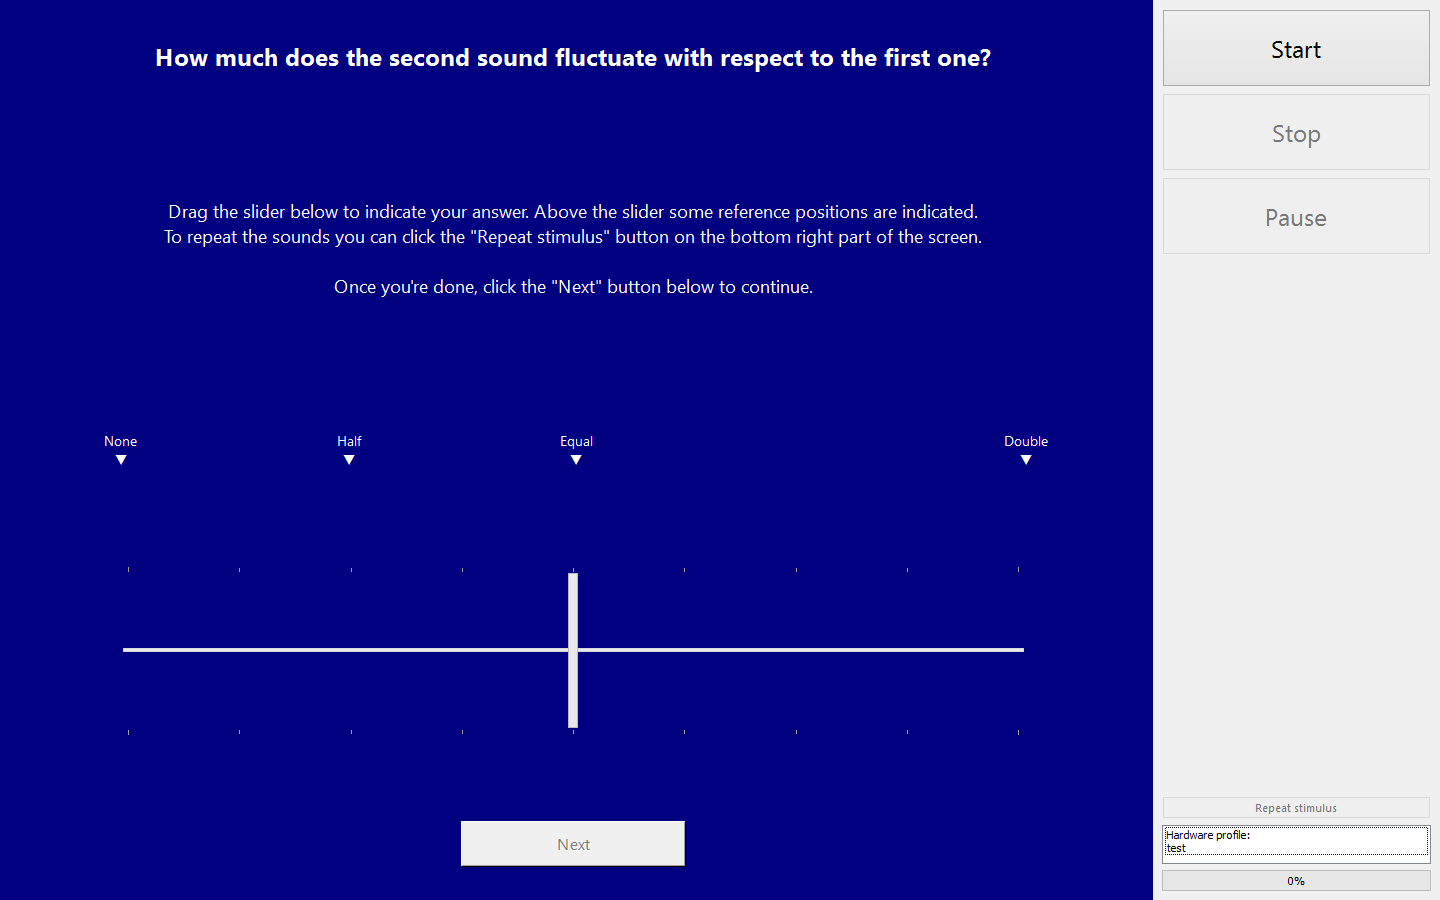
\includegraphics[width=\textwidth]{apex}
  \caption{Screenshot of the final experiment interface}
\label{fig:apex}
\end{figure}

\section{Results}

Talk about how data wil be processed and how it will be compared against
Fastl data.


\end{document}
